\documentclass{article}
\usepackage{graphicx}
\usepackage{fancyhdr}
\usepackage{listings}
\usepackage[utf8]{inputenc}
\usepackage{pgfplots}
\usepackage{booktabs}
\pgfplotsset{compat=1.14}

% 2 layers
\begin{filecontents}{128n2l-Loss.dat}
  X Step	Loss  	
  1 1   	3122.9219
  2 100		36.4435
  3 200		19.4324
  4 300		29.9501
  5 400		18.6390
  6 500   9.7420
\end{filecontents}

\begin{filecontents}{128n2l-Accuracy.dat}
  X Step	Accuracy  	
  1 1   	0.438
  2 100		0.898
  3 200		0.891
  4 300		0.844
  5 400		0.828
  6 500   0.875
\end{filecontents}

\begin{filecontents}{256n2l-Loss.dat}
  X Step	Loss  	
  1 1     8788.0879
  2 100   328.0475
  3 200   132.2209
  4 300   78.5238
  5 400   49.2364
  6 500   75.1907
\end{filecontents}

\begin{filecontents}{256n2l-Accuracy.dat}
  X Step	Accuracy  	
  1 1     0.453
  2 100   0.820
  3 200   0.875
  4 300   0.844
  5 400   0.836
  6 500   0.820
\end{filecontents}

\begin{filecontents}{512n2l-Loss.dat}
  X Step	Loss  	
  1 1     39196.4062
  2 100   1610.4182
  3 200   524.1964
  4 300   210.3122
  5 400   276.1759
  6 500   150.8354
\end{filecontents}

\begin{filecontents}{512n2l-Accuracy.dat}
  X Step	Accuracy  	
  1 1     0.359
  2 100   0.812
  3 200   0.883
  4 300   0.867
  5 400   0.812
  6 500   0.867
\end{filecontents}

% 3 layers
\begin{filecontents}{128n3l-Loss.dat}
  X Step	Loss  	
  1 1   	28933.5605
  2 100		741.4419
  3 200		255.7320
  4 300		325.6880
  5 400		244.8334
  6 500   130.3818
\end{filecontents}

\begin{filecontents}{128n3l-Accuracy.dat}
  X Step	Accuracy  	
  1 1   	0.344
  2 100		0.852
  3 200		0.914
  4 300		0.859
  5 400		0.867
  6 500   0.883
\end{filecontents}

\begin{filecontents}{256n3l-Loss.dat}
  X Step	Loss  	
  1 1     222537.9219
  2 100   4577.3066
  3 200   2686.8589
  4 300   2361.8943
  5 400   720.9211
  6 500   920.4222
\end{filecontents}

\begin{filecontents}{256n3l-Accuracy.dat}
  X Step	Accuracy  	
  1 1     0.359
  2 100   0.867
  3 200   0.875
  4 300   0.820
  5 400   0.875
  6 500   0.875
\end{filecontents}

\begin{filecontents}{512n3l-Loss.dat}
  X Step	Loss  	
  1 1     825527.0000
  2 100   15847.6143
  3 200   16547.9551
  4 300   4125.0908
  5 400   3149.9961
  6 500   5895.4766
\end{filecontents}

\begin{filecontents}{512n3l-Accuracy.dat}
  X Step	Accuracy  	
  1 1     0.422
  2 100   0.891
  3 200   0.836
  4 300   0.898
  5 400   0.891
  6 500   0.867
\end{filecontents}

% Testing Accuracy

\begin{filecontents}{testing-results.dat}
  X Neurons   2layers  3layers
  1 128       0.8734   0.8667
  2 256       0.8475   0.8635
  3 512       0.8438   0.8589
\end{filecontents}

\let\<\textless
\let\>\textgreater

\graphicspath{ {images/} }
\pagestyle{fancy}
\fancyhf{}
\rhead{Proyecto \#2}
\rfoot{P\'agina \thepage}

\begin{document}
\begin{titlepage}
  \centering
  {\scshape\LARGE Instituto Tecnol\'ogico de Costa Rica \par}
  \vspace{1cm}
  {\scshape\Large Inteligencia Articial\par}
  {\scshape\Large Proyecto \#2 - Redes Neuronales\par}
  \vspace{1.5cm}
  {\Large\itshape Sa\'ul Zamora\par}
  \vfill
  profesora\par
  Mar\'ia Mora \textsc{}

  \vfill

% Bottom of the page
  % {\large \today\par}
\end{titlepage}

\section{Abstract}

Artificial neural networks or simply “neural nets” go by many names such as connectionist models, parallel distributed processing models, and neuromorphic systems. Whatever terminology it may be, they all attempt to borrow the structure and running way of the biological nervous system based on our present understanding of it. Instead of performing a program consisting of instructions sequentially as in a von Neumann computer, artificial neural nets have their structures in dense interconnection of simple computational elements— the artificial neurons or simply “neurons”, and operate the massive computational elements in parallel to achieve high performance speed.

\section{Introduction}

An Artificial Neural Network (ANN) is a computational model that is inspired by the way biological neural networks in the human brain process information. Artificial Neural Networks have generated a lot of excitement in Machine Learning research and industry, thanks to many breakthrough results in speech recognition, computer vision and text processing. In this blog post we will try to develop an understanding of a particular type of Artificial Neural Network called the Multi Layer Perceptron.

\subsection{A Single Neuron}

The basic unit of computation in a neural network is the \textbf{neuron}, often called a \textbf{node} or \textbf{unit}. It receives input from some other nodes, or from an external source and computes an output. Each input has an associated \textbf{weight} (w), which is assigned on the basis of its relative importance to other inputs. The node applies a function \emph{\textbf{f}} (defined in Figure~\ref{neuron}) to the weighted sum of its inputs as shown in Figure~\ref{neuron}.

\begin{figure}[!h]
	\centering
		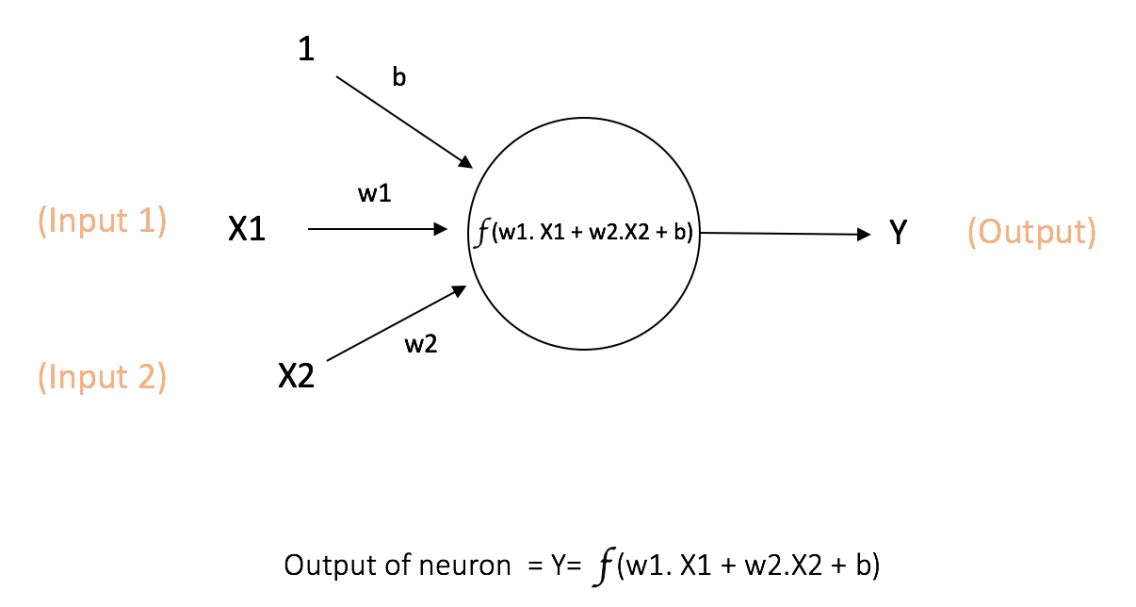
\includegraphics[width=\columnwidth]{images/neuron.png}
		\caption{A single neuron}\label{neuron}
	\label{fig:graph}
\end{figure}

The above network takes numerical inputs \textbf{X1} and \textbf{X2} and has weights \textbf{w1} and \textbf{w2} associated with those inputs. Additionally, there is another input \textbf{1} with weight \textbf{b} (called the \textbf{Bias}) associated with it. We will learn more details about role of the bias later.

The output Y from the neuron is computed as shown in the Figure~\ref{neuron}. The function \emph{\textbf{f}} is non-linear and is called the \textbf{Activation Function}. The purpose of the activation function is to introduce non-linearity into the output of a neuron. This is important because most real world data is non linear and we want neurons to learn these non linear representations.

Every activation function (or non-linearity) takes a single number and performs a certain fixed mathematical operation on it. There are several activation functions you may encounter in practice:

\begin{itemize}
  \item \textbf{Sigmoid}: takes a real-valued input and squashes it to range between 0 and 1
  \item \textbf{tanh}: takes a real-valued input and squashes it to the range [-1, 1]
  \item \textbf{ReLu}: ReLU stands for Rectified Linear Unit. It takes a real-valued input and thresholds it at zero (replaces negative values with zero)
\end{itemize}

\begin{figure}[!h]
	\centering
		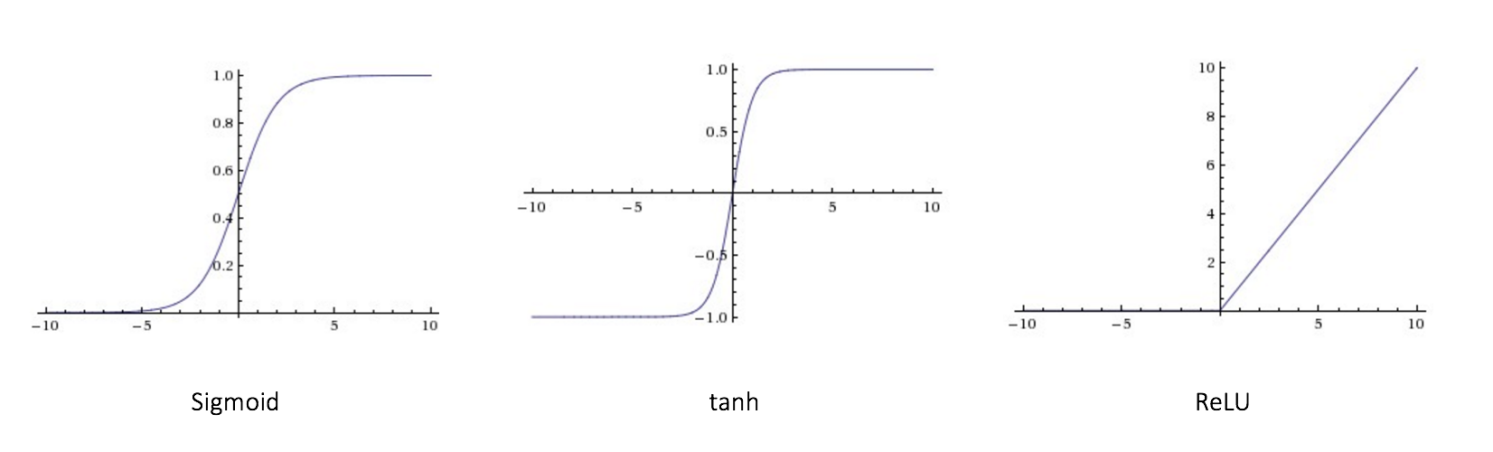
\includegraphics[width=\columnwidth]{images/activation-functions.png}
		\caption{Different activation functions}\label{activation-functions}
	\label{fig:graph}
\end{figure}

\section{Methods}

\subsection{Neural Network}

This project implements a feedforward neural network, which is the first and simplest type of artificial neural network devised. It contains multiple neurons (nodes) arranged in \textbf{layers}. Nodes from adjacent layers have \textbf{connections} or \textbf{edges} between them. All these connections have \textbf{weights} associated with them.

\begin{figure}[!ht]
	\centering
		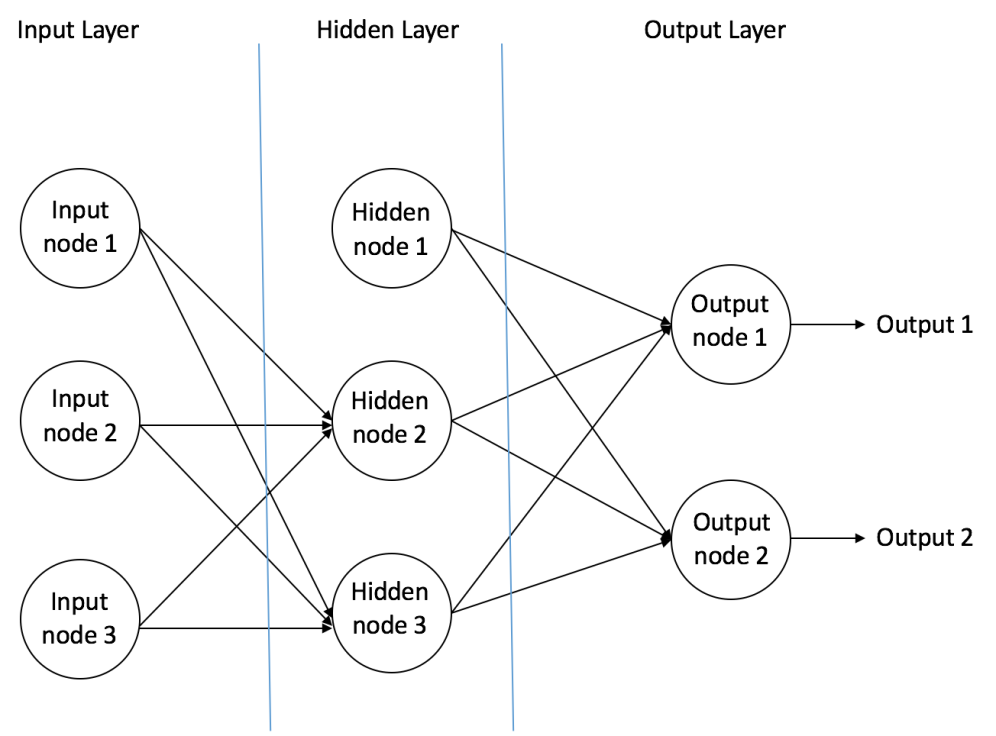
\includegraphics[width=\columnwidth]{images/feedforward-ff.png}
		\caption{Example of feedforward neural network}\label{feedforward-ff}
	\label{fig:graph}
\end{figure}

A feedforward neural network can consist of three types of nodes:

\begin{itemize}
  \item \textbf{Input Nodes}: provide information from the outside world to the network and are together referred to as the “Input Layer”. No computation is performed in any of the Input nodes – they just pass on the information to the hidden nodes.
  \item \textbf{Hidden Nodes}: they have no direct connection with the outside world (hence the name “hidden”). They perform computations and transfer information from the input nodes to the output nodes. A collection of hidden nodes forms a “Hidden Layer”. While a feedforward network will only have a single input layer and a single output layer, it can have zero or multiple Hidden Layers.
  \item \textbf{Output Nodes}: they are collectively referred to as the “Output Layer” and are responsible for computations and transferring information from the network to the outside world.
\end{itemize}

In a feedforward network, the information moves in only one direction – forward – from the input nodes, through the hidden nodes (if any) and to the output nodes. There are no cycles or loops in the network (this property of feed forward networks is different from Recurrent Neural Networks in which the connections between the nodes form a cycle).

\subsubsection{Multilayer Perceptron}

A Multi Layer Perceptron (MLP) has one or more hidden layers. We will only discuss Multi Layer Perceptrons as they are the ones implemented in this project. An MLP contains one or more hidden layers (apart from one input and one output layer).  While a single layer perceptron can only learn linear functions, a multi layer perceptron can also learn non – linear functions.

\begin{figure}[!h]
	\centering
		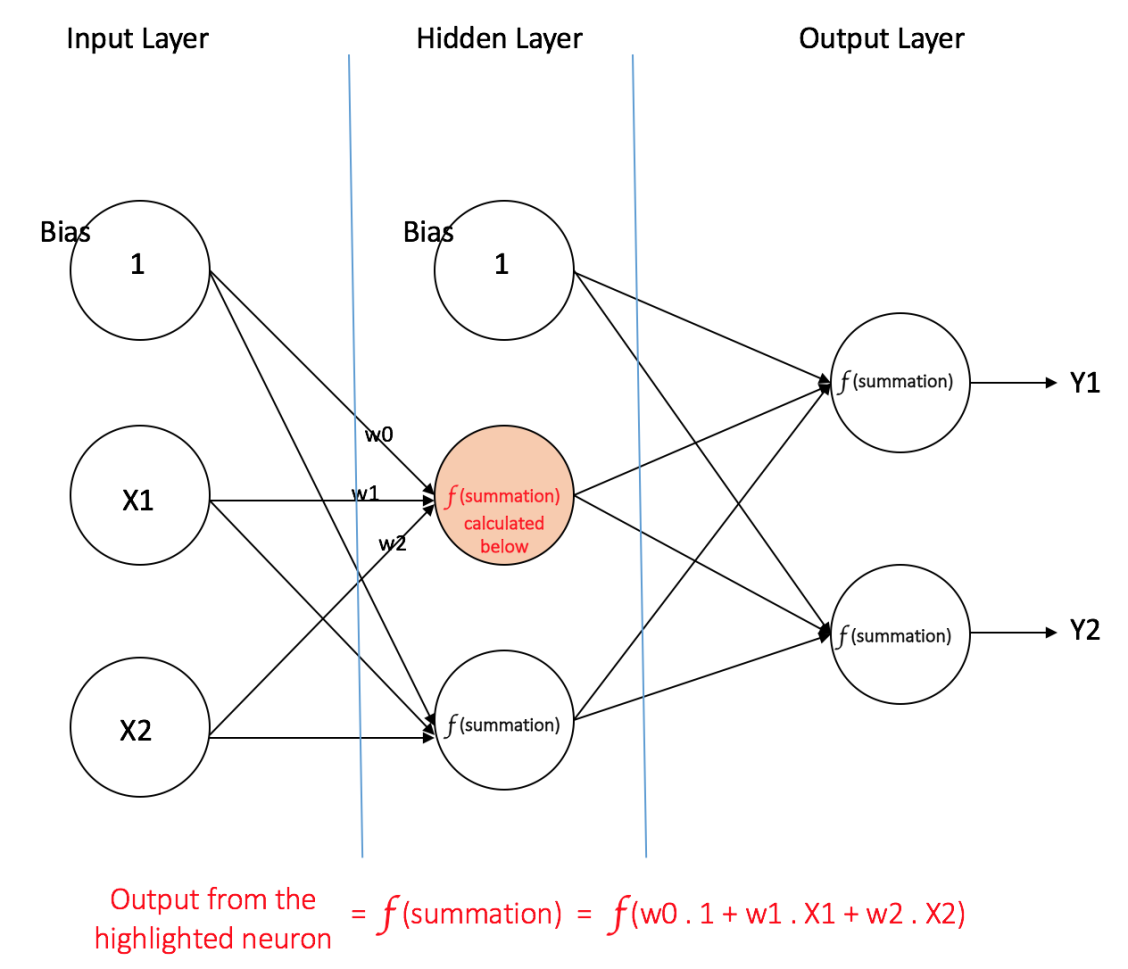
\includegraphics[width=\columnwidth]{images/mlp.png}
		\caption{Example a multi layer perceptron having one hidden layer}\label{mlp}
	\label{fig:graph}
\end{figure}

Figure~\ref{mlp} shows a multi layer perceptron with a single hidden layer. Note that all connections have weights associated with them, but only three weights (w0, w1, w2) are shown in the figure.

\begin{itemize}
  \item \textbf{Input Layer}: The Input layer has three nodes. The Bias node has a value of 1. The other two nodes take X1 and X2 as external inputs (which are numerical values depending upon the input dataset). As discussed above, no computation is performed in the Input layer, so the outputs from nodes in the Input layer are 1, X1 and X2 respectively, which are fed into the Hidden Layer.

  \item \textbf{Hidden Layer}: The Hidden layer also has three nodes with the Bias node having an output of 1. The output of the other two nodes in the Hidden layer depends on the outputs from the Input layer (1, X1, X2) as well as the weights associated with the connections (edges). Figure 4 shows the output calculation for one of the hidden nodes (highlighted). Similarly, the output from other hidden node can be calculated. Remember that f refers to the activation function. These outputs are then fed to the nodes in the Output layer.
  \item \textbf{Output Layer}: The Output layer has two nodes which take inputs from the Hidden layer and perform similar computations as shown for the highlighted hidden node. The values calculated (Y1 and Y2) as a result of these computations act as outputs of the Multi Layer Perceptron.
\end{itemize}

Given a set of features $X = (x1, x2, …)$ and a target \textbf{y}, a MLP can learn the relationship between the features and the target, for either classification or regression.

\subsection{TensorFlow}

This project uses TensorFlow to help process the training and test images to feed the neural network.

TensorFlow is an open-source software library for dataflow programming across a range of tasks. It is a symbolic math library, and is also used for machine learning applications such as neural networks. It is used for both research and production at Google.

TensorFlow is Google Brain's second-generation system. Version 1.0.0 was released on February 11, 2017. While the reference implementation runs on single devices, TensorFlow can run on multiple CPUs and GPUs (with optional CUDA and SYCL extensions for general-purpose computing on graphics processing units). TensorFlow is available on 64-bit Linux, macOS, Windows, and mobile computing platforms including Android and iOS.

Its flexible architecture allows for the easy deployment of computation across a variety of platforms (CPUs, GPUs, TPUs), and from desktops to clusters of servers to mobile and edge devices.

TensorFlow computations are expressed as stateful dataflow graphs. The name TensorFlow derives from the operations that such neural networks perform on multidimensional data arrays. These arrays are referred to as "tensors". In June 2016, Dean stated that 1,500 repositories on GitHub mentioned TensorFlow, of which only 5 were from Google.

\subsection{MNIST}

The MNIST database (Modified National Institute of Standards and Technology database) is a large database of handwritten digits that is commonly used for training various image processing systems. The database is also widely used for training and testing in the field of machine learning. It was created by "re-mixing" the samples from NIST's original datasets. The creators felt that since NIST's training dataset was taken from American Census Bureau employees, while the testing dataset was taken from American high school students, it was not well-suited for machine learning experiments. Furthermore, the black and white images from NIST were normalized to fit into a 28x28 pixel bounding box and anti-aliased, which introduced grayscale levels.

The MNIST database contains 60,000 training images and 10,000 testing images. Half of the training set and half of the test set were taken from NIST's training dataset, while the other half of the training set and the other half of the test set were taken from NIST's testing dataset. There have been a number of scientific papers on attempts to achieve the lowest error rate; one paper, using a hierarchical system of convolutional neural networks, manages to get an error rate on the MNIST database of 0.23\%. The original creators of the database keep a list of some of the methods tested on it. In their original paper, they use a support vector machine to get an error rate of 0.8\%. An extended dataset similar to MNIST called EMNIST has been published in 2017, which contains 240,000 training images, and 40,000 testing images of handwritten digits and characters.

\section{Results}

This project implemented 6 different configurations for the MLP, and the results show as follows:

\begin{itemize}
  \item 128 neurons per layer, 2 layers
  \item 256 neurons per layer, 2 layers
  \item 512 neurons per layer, 2 layers
  \item 128 neurons per layer, 3 layers
  \item 256 neurons per layer, 3 layers
  \item 512 neurons per layer, 3 layers
\end{itemize}

\newpage

\subsection{Neural Network Trainning Results}

% 128 neurons per layer, 2 layers
\begin{table}[!h]
  \centering
  \begin{tabular}{@{}lll@{}}
  \toprule
  Step  & Batch Loss  & Training Accuracy \\ \midrule
  1     & 3122.9219   & 0.438 \\
  100   & 36.4435     & 0.898 \\
  200   & 19.4324     & 0.891 \\
  300   & 29.9501     & 0.844 \\
  400   & 18.6390     & 0.828 \\
  500   & 9.7420      & 0.875 \\ \bottomrule
  \end{tabular}
  \caption{128 neurons per layer, 2 layers}
\end{table}

\begin{table}[!h]
  \centering
  \begin{tabular}{@{}lll@{}}
  \toprule
  Step  & Batch Loss  & Training Accuracy \\ \midrule
  1     & 8788.0879   & 0.453 \\
  100   & 328.0475    & 0.820 \\
  200   & 132.2209    & 0.875 \\
  300   & 78.5238     & 0.844 \\
  400   & 49.2364     & 0.836 \\
  500   & 75.1907     & 0.820 \\ \bottomrule
  \end{tabular}
  \caption{256 neurons per layer, 2 layers}
\end{table}

\begin{table}[!h]
  \centering
  \begin{tabular}{@{}lll@{}}
  \toprule
  Step  & Batch Loss  & Training Accuracy \\ \midrule
  1     & 39196.4062  & 0.359 \\
  100   & 1610.4182   & 0.812 \\
  200   & 524.1964    & 0.883 \\
  300   & 210.3122    & 0.867 \\
  400   & 276.1759    & 0.812 \\
  500   & 150.8354    & 0.867 \\ \bottomrule
  \end{tabular}
  \caption{512 neurons per layer, 2 layers}
\end{table}

\newpage

\begin{table}[!h]
  \centering
  \begin{tabular}{@{}lll@{}}
  \toprule
  Step  & Batch Loss  & Training Accuracy \\ \midrule
  1     & 28933.5605  & 0.344 \\
  100   & 741.4419    & 0.852 \\
  200   & 255.7320    & 0.914 \\
  300   & 325.6880    & 0.859 \\
  400   & 244.8334    & 0.867 \\
  500   & 130.3818    & 0.883 \\ \bottomrule
  \end{tabular}
  \caption{128 neurons per layer, 3 layers}
\end{table}

\begin{table}[!h]
  \centering
  \begin{tabular}{@{}lll@{}}
  \toprule
  Step  & Batch Loss  & Training Accuracy \\ \midrule
  1     & 222537.9219 & 0.359 \\
  100   & 4577.3066   & 0.867 \\
  200   & 2686.8589   & 0.875 \\
  300   & 2361.8943   & 0.820 \\
  400   & 720.9211    & 0.875 \\
  500   & 920.4222    & 0.875 \\ \bottomrule
  \end{tabular}
  \caption{256 neurons per layer, 3 layers}
\end{table}

\begin{table}[!h]
  \centering
  \begin{tabular}{@{}lll@{}}
  \toprule
  Step  & Batch Loss  & Training Accuracy \\ \midrule
  1     & 825527.0000 & 0.422 \\
  100   & 15847.6143  & 0.891 \\
  200   & 16547.9551  & 0.836 \\
  300   & 4125.0908   & 0.898 \\
  400   & 3149.9961   & 0.891 \\
  500   & 5895.4766   & 0.867 \\ \bottomrule
  \end{tabular}
  \caption{512 neurons per layer, 3 layers}
\end{table}

\newpage

\begin{figure}[!h]
  \centering
  \begin{tikzpicture}
  \begin{axis}[
  axis lines=middle,
  ymin=0,
  x label style={at={(current axis.right of origin)},anchor=north, below=10mm},
  title={\textit{\textbf{128 neurons per layer, 2 layers - Batch Loss}}},
      xlabel=Step,
    ylabel=Batch Loss,
    xticklabel style = {rotate=30,anchor=east},
     enlargelimits = false,
    xticklabels from table={128n2l-Loss.dat}{Step},xtick=data]
  \addplot[red,thick,mark=square*] table [y=Loss,x=X]{128n2l-Loss.dat};
  \end{axis}
  \end{tikzpicture}
\end{figure}

\begin{figure}[!h]
  \centering
  \begin{tikzpicture}
  \begin{axis}[
  axis lines=middle,
  ymin=0,
  x label style={at={(current axis.right of origin)},anchor=north, below=10mm},
  title={\textit{\textbf{128 neurons per layer, 2 layers - Testing Accuracy}}},
      xlabel=Step,
    ylabel=Testing Accuracy,
    xticklabel style = {rotate=30,anchor=east},
     enlargelimits = false,
    xticklabels from table={128n2l-Accuracy.dat}{Step},xtick=data]
  \addplot[blue,thick,mark=square*] table [y=Accuracy,x=X]{128n2l-Accuracy.dat};
  \end{axis}
  \end{tikzpicture}
\end{figure}

\newpage

% 256 neurons per layer, 2 layers

\begin{figure}[!h]
  \centering
  \begin{tikzpicture}
  \begin{axis}[
  axis lines=middle,
  ymin=0,
  x label style={at={(current axis.right of origin)},anchor=north, below=10mm},
  title={\textit{\textbf{256 neurons per layer, 2 layers - Batch Loss}}},
      xlabel=Step,
    ylabel=Batch Loss,
    xticklabel style = {rotate=30,anchor=east},
     enlargelimits = false,
    xticklabels from table={256n2l-Loss.dat}{Step},xtick=data]
  \addplot[red,thick,mark=square*] table [y=Loss,x=X]{256n2l-Loss.dat};
  \end{axis}
  \end{tikzpicture}
\end{figure}

\begin{figure}[!h]
  \centering
  \begin{tikzpicture}
  \begin{axis}[
  axis lines=middle,
  ymin=0,
  x label style={at={(current axis.right of origin)},anchor=north, below=10mm},
  title={\textit{\textbf{256 neurons per layer, 2 layers - Testing Accuracy}}},
      xlabel=Step,
    ylabel=Testing Accuracy,
    xticklabel style = {rotate=30,anchor=east},
     enlargelimits = false,
    xticklabels from table={256n2l-Accuracy.dat}{Step},xtick=data]
  \addplot[blue,thick,mark=square*] table [y=Accuracy,x=X]{256n2l-Accuracy.dat};
  \end{axis}
  \end{tikzpicture}
\end{figure}

\newpage

% 512 neurons per layer, 2 layers

\begin{figure}[!h]
  \centering
  \begin{tikzpicture}
  \begin{axis}[
  axis lines=middle,
  ymin=0,
  x label style={at={(current axis.right of origin)},anchor=north, below=10mm},
  title={\textit{\textbf{512 neurons per layer, 2 layers - Batch Loss}}},
      xlabel=Step,
    ylabel=Batch Loss,
    xticklabel style = {rotate=30,anchor=east},
     enlargelimits = false,
    xticklabels from table={512n2l-Loss.dat}{Step},xtick=data]
  \addplot[red,thick,mark=square*] table [y=Loss,x=X]{512n2l-Loss.dat};
  \end{axis}
  \end{tikzpicture}
\end{figure}

\begin{figure}[!h]
  \centering
  \begin{tikzpicture}
  \begin{axis}[
  axis lines=middle,
  ymin=0,
  x label style={at={(current axis.right of origin)},anchor=north, below=10mm},
  title={\textit{\textbf{512 neurons per layer, 2 layers - Testing Accuracy}}},
      xlabel=Step,
    ylabel=Testing Accuracy,
    xticklabel style = {rotate=30,anchor=east},
     enlargelimits = false,
    xticklabels from table={512n2l-Accuracy.dat}{Step},xtick=data]
  \addplot[blue,thick,mark=square*] table [y=Accuracy,x=X]{512n2l-Accuracy.dat};
  \end{axis}
  \end{tikzpicture}
\end{figure}

\newpage

% 128 neurons per layer, 3 layers

\begin{figure}[!h]
  \centering
  \begin{tikzpicture}
  \begin{axis}[
  axis lines=middle,
  ymin=0,
  x label style={at={(current axis.right of origin)},anchor=north, below=10mm},
  title={\textit{\textbf{128 neurons per layer, 3 layers - Batch Loss}}},
      xlabel=Step,
    ylabel=Batch Loss,
    xticklabel style = {rotate=30,anchor=east},
     enlargelimits = false,
    xticklabels from table={128n3l-Loss.dat}{Step},xtick=data]
  \addplot[red,thick,mark=square*] table [y=Loss,x=X]{128n3l-Loss.dat};
  \end{axis}
  \end{tikzpicture}
\end{figure}

\begin{figure}[!h]
  \centering
  \begin{tikzpicture}
  \begin{axis}[
  axis lines=middle,
  ymin=0,
  x label style={at={(current axis.right of origin)},anchor=north, below=10mm},
  title={\textit{\textbf{128 neurons per layer, 3 layers - Testing Accuracy}}},
      xlabel=Step,
    ylabel=Testing Accuracy,
    xticklabel style = {rotate=30,anchor=east},
     enlargelimits = false,
    xticklabels from table={128n3l-Accuracy.dat}{Step},xtick=data]
  \addplot[blue,thick,mark=square*] table [y=Accuracy,x=X]{128n3l-Accuracy.dat};
  \end{axis}
  \end{tikzpicture}
\end{figure}

\newpage

% 256 neurons per layer, 3 layers

\begin{figure}[!h]
  \centering
  \begin{tikzpicture}
  \begin{axis}[
  axis lines=middle,
  ymin=0,
  x label style={at={(current axis.right of origin)},anchor=north, below=10mm},
  title={\textit{\textbf{256 neurons per layer, 3 layers - Batch Loss}}},
      xlabel=Step,
    ylabel=Batch Loss,
    xticklabel style = {rotate=30,anchor=east},
     enlargelimits = false,
    xticklabels from table={256n3l-Loss.dat}{Step},xtick=data]
  \addplot[red,thick,mark=square*] table [y=Loss,x=X]{256n3l-Loss.dat};
  \end{axis}
  \end{tikzpicture}
\end{figure}

\begin{figure}[!h]
  \centering
  \begin{tikzpicture}
  \begin{axis}[
  axis lines=middle,
  ymin=0,
  x label style={at={(current axis.right of origin)},anchor=north, below=10mm},
  title={\textit{\textbf{256 neurons per layer, 3 layers - Testing Accuracy}}},
      xlabel=Step,
    ylabel=Testing Accuracy,
    xticklabel style = {rotate=30,anchor=east},
     enlargelimits = false,
    xticklabels from table={256n3l-Accuracy.dat}{Step},xtick=data]
  \addplot[blue,thick,mark=square*] table [y=Accuracy,x=X]{256n3l-Accuracy.dat};
  \end{axis}
  \end{tikzpicture}
\end{figure}

\newpage

% 512 neurons per layer, 3 layers

\begin{figure}[!h]
  \centering
  \begin{tikzpicture}
  \begin{axis}[
  axis lines=middle,
  ymin=0,
  x label style={at={(current axis.right of origin)},anchor=north, below=10mm},
  title={\textit{\textbf{512 neurons per layer, 3 layers - Batch Loss}}},
      xlabel=Step,
    ylabel=Batch Loss,
    xticklabel style = {rotate=30,anchor=east},
     enlargelimits = false,
    xticklabels from table={512n3l-Loss.dat}{Step},xtick=data]
  \addplot[red,thick,mark=square*] table [y=Loss,x=X]{512n3l-Loss.dat};
  \end{axis}
  \end{tikzpicture}
\end{figure}

\begin{figure}[!h]
  \centering
  \begin{tikzpicture}
  \begin{axis}[
  axis lines=middle,
  ymin=0,
  x label style={at={(current axis.right of origin)},anchor=north, below=10mm},
  title={\textit{\textbf{512 neurons per layer, 3 layers - Testing Accuracy}}},
      xlabel=Step,
    ylabel=Testing Accuracy,
    xticklabel style = {rotate=30,anchor=east},
     enlargelimits = false,
    xticklabels from table={512n3l-Accuracy.dat}{Step},xtick=data]
  \addplot[blue,thick,mark=square*] table [y=Accuracy,x=X]{512n3l-Accuracy.dat};
  \end{axis}
  \end{tikzpicture}
\end{figure}

\newpage

\subsection{Neural Network Testing Results}

\begin{table}[!h]
  \centering
  \begin{tabular}{@{}lll@{}}
  \toprule
  Neurons   & 2 layers  & 3 layers \\ \midrule
  128       & 0.8734    & 0.8667 \\
  256       & 0.8475    & 0.8635 \\
  512       & 0.8438    & 0.8589 \\ \bottomrule
  \end{tabular}
  \caption{Testing Accuracy}
\end{table}

\begin{figure}[!h]
  \centering
  \begin{tikzpicture}
  \begin{axis}[
  axis lines=middle,
  ymin=0.8, ymax=0.9,
  x label style={at={(current axis.right of origin)},anchor=north, below=10mm},
  title={\textit{\textbf{Testing Accuracy Results}}},
      xlabel=Neurons,
    ylabel=Accuracy,
    xticklabel style = {rotate=30,anchor=east},
     enlargelimits = false,
    xticklabels from table={testing-results.dat}{Neurons},xtick=data]
  \addplot[red,thick,mark=square*] table [y=2layers,x=X]{testing-results.dat};
  \addlegendentry{2 layers}
  \addplot[blue,thick,mark=square*] table [y=3layers,x=X]{testing-results.dat};
  \addlegendentry{3 layers}
  \end{axis}
  \end{tikzpicture}
\end{figure}

\section{Conclusions}

\begin{itemize}
  \item Effects of increasing the number of neurons in both 2 and 3 layered NN:
  \begin{itemize}
    \item Trainning accuracy does not suffers much.
    \item Batch loss increases massively.
    \item Testing accuracy decreases.
  \end{itemize}
  \item By adding an extra layer to the neural network, the impact of adding extra neurons to the layers is much less than with only two layers.
\end{itemize}

\begin{thebibliography}{9}
  \bibitem{article}
  Barbara J. Hoogenboom, R. (2018). HOW TO WRITE A SCIENTIFIC ARTICLE. [online] PubMed Central (PMC).
  Available at: \texttt{https://www.ncbi.nlm.nih.gov/pmc/articles/PMC3474301/}

  \bibitem{nn}
  the data science blog. (2018). A Quick Introduction to Neural Networks. [online]
  Available at: \texttt{https://ujjwalkarn.me/2016/08/09/quick-intro-neural-networks/}

  \bibitem{tensorflow}
  En.wikipedia.org. (2018). TensorFlow. [online]
  Available at: \texttt{https://en.wikipedia.org/wiki/TensorFlow}
  
\end{thebibliography}

\end{document}
